\chapter{Implementacja}
\section{Interfejs użytkownika}
Z wykorzystaniem wbudowanych w Godot węzłów zbudowane zostały interfejsy zaprojektowane w sekcji \ref{sec:interface_design}. Problematyczne okazało się dostosowanie układu tak, aby przy zmianie rozmiaru okna elementy nie nachodziły na siebie. Dodatkowo, przy skalowaniu okna nie ma możliwości dynamicznego dostosowania wielkości czcionki do wielkości kontrolki w której się znajduje.  Było to szczególnym problemem podczas testowania oprogramowania, kiedy często należało uruchamiać kilka instancji na jednym ekranie. W domyślnym użytkowaniu gry taki problem nie powinien występować, ponieważ gra będzie rozgrywana na pełnym ekranie.

W celu ustawienia kontrolek w odpowiednich miejscach i w odpowiednich relacjach wykorzystane zostały węzły kontenerowe: \texttt{VBoxContainer}, \texttt{HBoxContainer} i \texttt{GridContainer}.

Innym problemem napotkanym podczas implementacji okazało się przełączanie scen. Problem był zauważalny między rundami, gdzie menu wyboru kart nie było wyświetlane mimo, że powinno było. Problemem okazał się być fakt, iż przełączenie sceny nie dzieje się od razu. Jest ono odsunięte w czasie na klatkę po wykonaniu całej funkcji. Dodatkowo zmiana sceny nie powoduje zakończenia funkcji. Doprowadziło to do sytuacji, w której scena była zmieniana wielokrotnie w jednym wykonaniu. Po odnalezieniu powodu takiego zachowania w dokumentacji rozwiązaniem było opuszczanie funkcji słowem kluczowym \texttt{return} po zamianie sceny.

HUD gracza podzielono na podelementy. Oddzielnie przygotowano scenę informacji własnych gracza, oddzielnie zaś scenę informacji innych graczy. Sceny te połączono z danymi na temat żywotności i liczby pocisków poszczególnych graczy przy pomocy sygnałów. Sceny z informacjami innych graczy tworzone i dodawane są do gry w momencie rozesłania sygnału rozpoczęcia rozgrywki. Pełna scena HUD dodana została do sceny gracza. Sprawia to, że jest ona stale dostępna w oknie gry, jednak w przypadku uruchomienia sceny menu, HUD jest przez nią zasłaniany.

W menu kart, same karty również zostały przygotowane jako oddzielne sceny. Pozwala to na łatwe generowanie widoku z różnymi kartami, wyglądającymi tak samo. Jako tło karty ustawiony został węzeł \texttt{TextureRect}. Umożliwia to w przyszłości przygotowanie różnorodnych grafik dla różnych kart. W aktualnej implementacji. Podjęte zostały również próby umieszczenia na karcie informacji na temat modyfikowanych atrybutów, jednak potencjalnie duża możliwa ich liczba doprowadziła do decyzji o ukryciu ich przed graczem.

\section{Postać gracza}
Model postaci został przygotowany w programie Blender (rys. \ref{fig:model}). Ze względu na prostsze wykonanie, sam model wykonano w stylu \emph{low poly} (ang. mało wielokątów). Przygotowane zostały również materiały: pokrywający lufę i gąsienice oraz dwa pokrywające karoserię i wieżyczkę. W grze materiały kolorowe zostają zmodyfikowane tak, aby ich kolorem bazowym był ten wybrany przez gracza (rys. \ref{fig:model_green}). W celu wprowadzenia takiej modyfikacji należało zduplikować odpowiednie materiały (listing \ref{lst:changing_material}). Pominięcie tego kroku powodowało, że wszystkie modele w grze zmieniały kolor na ten sam. Dzieje się tak, ponieważ Godot domyślnie wykorzystuje zasoby jako współdizelone aby oszczędzać pamięć.

\begin{lstlisting}[language=python,caption=Kod zmieniający kolor materiału postaci gracza., label=lst:changing_material,basicstyle=\footnotesize\ttfamily]
func set_player_colour(new_colour: Color):
  player_colour = new_colour

  var body_mesh: Mesh = \$Model/Body/Body.mesh
  var tower_mesh: Mesh = \$Model/Head/Tower.mesh
  var barrel_mesh: Mesh = \$Model/Head/Barrel.mesh

  var body_material: SpatialMaterial 
    = preload("res://Resources/Models/BodyMaterial.material")
      .duplicate()
  var light_ring_material: SpatialMaterial 
    = preload("res://Resources/Models/BodyLight.material")
      .duplicate()
	
  body_material.albedo_color = new_colour
  light_ring_material.albedo_color = new_colour
  light_ring_material.emission = new_colour

  body_mesh.surface_set_material(0, body_material)
  tower_mesh.surface_set_material(0, body_material)
  tower_mesh.surface_set_material(1, light_ring_material)
  barrel_mesh.surface_set_material(0, body_material)

  if is_network_master():
    rset("puppet_player_colour", player_colour)
\end{lstlisting}

\begin{figure}
\centering
    \begin{subfigure}{.7\textwidth}
        \centering
        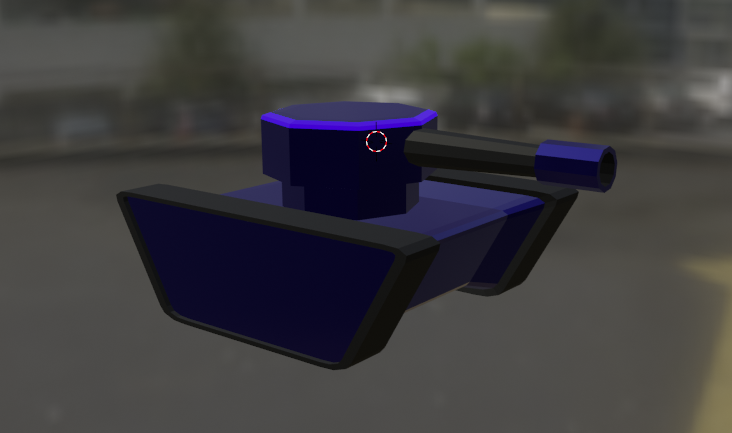
\includegraphics[width=.8\linewidth]{Images/development/model.png}
        \caption{Model w programie Blender.}
        \label{fig:model}
    \end{subfigure}
    
    \begin{subfigure}{.7\textwidth}
        \centering
        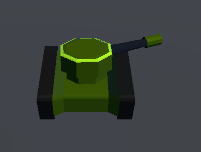
\includegraphics[width=.8\linewidth]{Images/development/model_green.png}
        \caption{Model o programowo zmienionych barwach.}
        \label{fig:model_green}
    \end{subfigure}
    \caption{Model czołgu.}
    \label{fig:both_models}
\end{figure}

Scena gracza jest rozszerzeniem węzła \texttt{KinematicBody}. Udostępnia on wiele metod związanych z ruchem i kolizjami, na przykład główną metodę wykorzystywaną do poruszania postaci: \texttt{move\_and\_slide}. Pozwala ona przemieszczać obiekty interpretując odpowiednio ich kolizje z innymi - przesuwając ciało wzdłuż płaszczyzny kolizji.


\begin{figure}
    \centering
    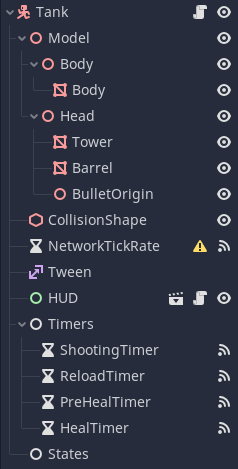
\includegraphics[width=.6\linewidth]{Images/development/tank_tree.png}
    \caption{Drzewo sceny postaci gracza.}
    \label{fig:player_scene_tree}
\end{figure}

Drzewo sceny gracza zawiera również inne istotne węzły (rys. \ref{fig:player_scene_tree}).

\begin{itemize}
    \item \textbf{\texttt{Model}} - Model postaci importowany z Blendera. Podzielony jest na trzy elementy wizualne: \texttt{Body}, reprezentujący główny kadłub, \texttt{Tower}, reprezentujący wieżyczkę i \texttt{Barrel}, reprezentujący lufę. Dwa ostatnie elementy są zgrupowane, ponieważ poruszają i obracają się wspólnie. Wraz z nimi zgrupowany jest \texttt{BulletOrigin} reprezentujący punkt w którym pociski są tworzone. Początkowo był on dzieckiem lufy, jednak wtedy aplikowane były do niego przekształcenia takie jak skalowanie i obroty, przeniesione z Blendera. Wpływały one na tworzone pociski, dlatego też został odłączony od lufy.  
    \item \textbf{\texttt{CollisionShape}} Kształt określający gdzie obiekty mogą wchodzić z czołgiem w kolizję. 
    \item \textbf{\texttt{NetworkTickRate}} Licznik czasu, na którego zakończenie wysyłane są dane na temat pozycji gracza. Odmierza 0.03 sekundy, co oznacza nieco ponad 33 razy na sekundę. Ze względu na działanie silnika zegar nie może uruchomić sygnału zakończenia częściej niż raz na klatkę, w związku z tym przy spowolnieniu aplikacji komunikacja internetowa również będzie odbywać się wolniej.
    \item \textbf{\texttt{HUD}} Opisany w sekcji \ref{sec:design_menu} element interfejsu użytkownika.
    \item \textbf{\texttt{Timers}} Zbiór liczników czasu potrzebnych w strzelaniu i leczeniu. \texttt{ShootingTimer} blokuje zbyt częste strzały. \texttt{ReloadTimer} odmierza czas przeładowania. \texttt{PreHealTimer} odmierza czas między otrzymaniem obrażeń a leczeniem. \texttt{HealTimer} określa jak częste będzie leczenie po jego rozpoczęciu. 
    \item \textbf{\texttt{States}} Węzeł zbierający w sobie wszelkie stany nadane graczowi jako efekt trafienia zmodyfikowanymi pociskami.
\end{itemize} 

\section{Implementacja mechanik}
\subsection{Strzelanie}
Do procesu strzelania dodane zostały odpowiednie elementy zgodnie z diagramem \ref{fig:shoot_flowchart}. Implementacja opiera się na licznikach czasu, które po zakończeniu odliczania zmieniają wartości odpowiednich zmiennych. Kod przedstawiający decyzje o strzale z uwzględnieniem buforowania został przedstawiony w listingu \ref{lst:shooting_impl}.

Po dodaniu możliwości zmiany szybkości pocisku kartami dotychczasowa implementacja przemieszczania okazała się niewystarczająca. Pocisk w implementacji prototypu był przenoszony na pozycję będacą przemieszczeniem o odpowiednio przemnożony wektor prędkości. W przypadku znacznego przyspieszenia pocisku jest to niewystarczająca implementacja. Prowadzi ona do ,,przenikania'' pocisków przez ściany. Kolizje między kaltkami nie są wykrywane, a pocisk może zostać przeniesiony bez jej wykrycia. W tym celu węzeł główny pocisku zmieniono z \texttt{Area} na \texttt{KinematicBody}. Umożliwiło to wykorzystanie funkcji \texttt{move\_and\_collide}. Przemieszcza ona obiekt o podany wektor, wykrywa jednak kolizje na drodze. Zwrócona przez funkcję kolizja może zostać w prosty sposób zinterpretowana pod kątem kolidującego obiektu, ruchu obu obiektów ale również punktu kolizji czy wektora normalnego płaszczyzny kolidującej w tym punkcie. Te dane okazały się przydatne w implementacji kolejnych kart znacznie upraszczając tworzone zachowania.  

\begin{lstlisting}[language=python,caption=Implementacja decyzji o dokonaniu strzału., label=lst:shooting_impl,basicstyle=\footnotesize\ttfamily]
if Input.is_action_just_pressed("MainAction") and can_shoot:
  if has_just_shot or is_reloading:
    shoot_buffer = SHOOT_BUFFER_FRAMES
  else:
    shoot()
elif shoot_buffer > 0: #shot buffering
  if is_reloading or has_just_shot:
    shoot_buffer -= 1
  else:
    shoot()
\end{lstlisting}

Do pocisku została dodana liczba pozostałych odbić. Po trafieniu przeszkody, jeżeli liczba odbić jest większ od zera zostaje ona zdekrementowana a następnie dochodzi do odbicia. Implementacja odbicia wykorzystuje wektor normalny płaszczyzny kolidującej. Jest on przekazywany do metody \texttt{Vector3.reflect}, która odbija wektor od zadanej wektorem normalnym powierzchni. W ten sposób zostaje obrócona prędkość pocisku. Następnie pocisk obracany jest w kierunku wskazywanym przez prędkość metodą \texttt{look\_at}.

\subsection{Komendy}
Wydarzenia po trafieniu zostały zaimplementowane jako komendy. W GDScript funkcje nie są obiektami jak w wielu innych językach, nie można również wyznaczyć wskaźnika na funkcję. W celu przechowywania funkcji jako zmiennej w obiekcie wykorzystano klasę \texttt{FuncRef}. Pozwala ona na stworzenie referencji na funkcję w \emph{konkretnym obiekcie}, która następnie może zostać wywołana. W związku z tym, aby takie funkcje móc wywoływać niezbędne jest zapewnienie istnienia obiektu, na którym będą wywoływane. W tym celu zostało stowrzone repozytorium komend. W klasie \texttt{CommandsRepository} zdefiniowane są wszystkie niezbędne funkcje oraz tworzone są wszystkie dostępne w grze komendy. Klasa ta zostaje autoładowana na początku działania aplikacji, jej instancja jest więc dostępna globalnie.

Określony został zestaw argumentów niezbędnych do stworzenia komend. Są to: pocisk wywołujący komendę, obiekt uczestniczący w kolizji oraz punkt kolizji. Te argumenty będą przekazywane przy każdym wywołaniu funkcji z komend. Możliwe jest dodanie kolejnych lub zmiana aktualnych argumentów poprzez stworzenie klasy dziedziczącej po \texttt{BaseCommand}, jednak wymagałoby to zmiany kodu obsługującego wywoływanie komend.


\subsection{Karty}
Została stworzona klasa bazowa dla kart, definiująca ich cztery atrybuty: nazwę, opis, zmiany atrybutów i listę komend. Te atrybuty zostały dokładniej opisane w sekcji \ref{sec:cards_design}. Została również dodana metoda aplikująca wszystkie zmiany do gracza, przedstawiona w listingu \ref{lst:attach_to_player}

\begin{lstlisting}[language=python,caption=Metoda aplikująca zmiany atrybutów gracza., label=lst:attach_to_player,basicstyle=\footnotesize\ttfamily]
func attach_to_player(player: KinematicBody):
  for key in attribute_changes.keys():
    if player.get(key) != null:
      match attribute_changes[key][0]:
        "*":
          player[key] *= attribute_changes[key][1]
        "+":
          player[key] += attribute_changes[key][1]
  if player.get("bullet_on_hit") != null:
    player["bullet_on_hit"].append_array(on_hit)
  if player.get("cards") != null:
    player["cards"].append(self)
\end{lstlisting}

Dla kart, podobnie jak dla komend, stworzone zostało autoładowane repozytorium \texttt{CardsRepository}. Tworzone są w nim obiekty każdej z kart. Udostępnia ono również metody do losowania kart, w szczególności do wylosowania trzech kart w celu wyboru między rundami.  

\section{Obiekty globalne}
W ustawieniach projektu skonfigurowane zostały obiekty autoładowane odpowiedzialne za zarządzanie różnymi aspektami rozgrywki. W poprzednich sekcjach opisane zostały repozytoria komend i kart. 

Kolejnym obiektem globalnym jest \texttt{GameState} - odpowiedzialny za zarządzanie stanem gry. Zapisane są w nim najważniejsze dane użytkowników potrzebne do prezentacji w menu. Zapisywane są tam również postępy w rozgrywce - docelowa lcizba punktów zwycięstwa, aktualna liczba punktów każdego z graczy, lista wyeliminowanych w aktualnej rundzie graczy oraz zwycięzca ostatniej rundy. Udostępnione są tu również metody pozwalające zarządzać postępem rund - rozpoczynanie i zakańczanie rund, znajdowanie najsłabszych graczy i zwycięzcy oraz zbieranie danych na temat wybieranych przez graczy kart.

Skrypt globalny \texttt{Network} odpowiada za zarządzanie połączeniami sieciowymi. Udostępnia metody pozwalające tworzyć serwer oraz do niego dołączać, odłączać się od sieci. Umożliwia również nazywanie obiektów sieciowych w sposób synchronizowany pomiędzy klientami. Skrypt ten jest również połączony z najważniejszymi sygnałami sieciowymi emitowanymi przez drzewo gry. 

Obiekt \texttt{Global} odpowiedzialny jest za zarządzanie najważniejszymi obiektami. Udostępnia też wiele metod upraszczających tworzenie nowych węzłów.

Węzeł globalny \texttt{PersistentNodes} nie ma przypisanego skryptu. Jako jego dzieci zapisywane są tworzone w trakcie gry obiekty dynamiczne, których częste tworzenie może znacznie obciążać komputer. Tutaj zapisywane są obiekty postaci graczy i pociski. 

\section{Testy}
Z wykorzystaniem narzędzia GUT stworzone zostały testy skryptów globalnych. Skrypty \texttt{Global}, \texttt{Network} i \texttt{GameState} zostały przetestowane integracyjnie i jednostkowo. Sumarycznie zostało napisanych 13 testów skłądających się z 40 asercji (rys. \ref{fig:test_results}).

\begin{figure}
    \centering
    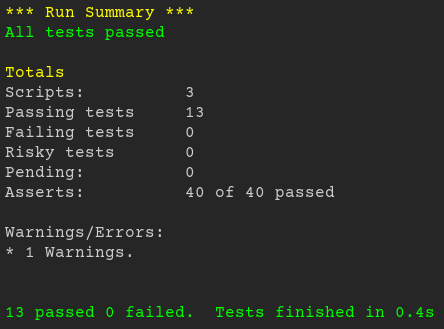
\includegraphics[width=.5\linewidth]{Images/development/tests_result.png}
    \caption{Wyniki uruchomienia testów automatycznych.}
    \label{fig:test_results}
\end{figure}

Przeprowadzone zostały również testy manualne zarówno wielu instancji aplikacji na jednym komputerze jak i połączenia po sieci lokalnej LAN. W wyniku testów odkryto wiele błędów, większość z których udało się naprawić. Przykładem takiego błędu był błąd, który sprawiał, że połączenia serwera oraz dane gry nie były usuwane po zakończeniu gry. Z tego powodu kolejne uruchomienie gry powodowało wskazanie, że większa liczba graczy jest podłączona do serwera niż w rzeczywistości. Naprawienie tego błędu wymagało pełnego czyszczenia stanu gry po każdym zakończeniu rozgrywki.

